% !TEX root = Thesis Template University of Insubria/tesi.tex
\documentclass[a4paper, 11pt, twoside]{book}
\usepackage[a4paper]{geometry}
\usepackage{lmodern}
\usepackage[italian]{babel}
\usepackage{textcomp}
\usepackage{color}
\usepackage{url}
\usepackage{amsfonts}
\usepackage{float}
\usepackage{booktabs}
\usepackage{longtable}
\usepackage{makeidx}
\usepackage{fancyhdr}
\usepackage[times]{quotchap}
\usepackage{multirow}
\usepackage{version}
\usepackage{abstract}
\usepackage{listings}
\usepackage{color}
\usepackage{xcolor}
\usepackage{listings}

\definecolor{gray}{rgb}{0.9,0.9,0.9}

%%modifiche per il codice
\lstdefinestyle{basic}{  
  basicstyle=\footnotesize\ttfamily,
  numbers=left,
  numberstyle=\tiny\color{orange}\ttfamily,
  numbersep=5pt,
  backgroundcolor=\color{white},
  showspaces=false,
  showstringspaces=false,
  showtabs=false,
  frame=single,
  rulecolor=\color{black},
  captionpos=b,
  keywordstyle=\color{blue}\bf,
  commentstyle=\color{gray},
  stringstyle=\color{green},
  keywordstyle={[2]\color{red}\bf},
}


\lstdefinelanguage{DebianBash}
{
  morekeywords={cd, apt-get, service, vagrant, docker-compose, docker, &&, 
    time, curl, sudo, echo, set, psql, EOF, cat, if, then, echo, chmod, until, do,
    sleep, done, firefox, git , pip, shovel, honcho},
  morecomment=[l]{\#},
  morestring=[b]",
  alsodigit={-},
  alsoletter={&}
}

\lstdefinestyle{customjava}{
  	language=Java,
  	frame=tlrb,
  	aboveskip=3mm,
  	belowskip=6mm,
  	showstringspaces=false,
  	columns=flexible,
  	basicstyle={\small\ttfamily},
  	numbers=left,
    numberstyle=\tiny\color{orange}\ttfamily,
    numbersep=5pt,
  	keywordstyle=\color{purple},
  	commentstyle=\color{orange},
  	stringstyle=\color{blue},
  	breaklines=true,
  	breakatwhitespace=true
  	tabsize=3
}

\lstdefinestyle{custompython}{
  	language=Python,
  	frame=tlrb,
  	aboveskip=3mm,
  	belowskip=6mm,
  	showstringspaces=false,
  	columns=flexible,
  	basicstyle={\small\ttfamily},
  	numbers=left,
    numberstyle=\tiny\color{orange}\ttfamily,
    numbersep=5pt,
  	keywordstyle=\color{purple},
  	commentstyle=\color{orange},
  	stringstyle=\color{blue},
  	breaklines=true,
  	breakatwhitespace=true
  	tabsize=3
}

\lstset{
  language=Python,
  basicstyle=\small\ttfamily,
  numbers=left,
  numberstyle=\tiny,
  frame=tb,
  columns=fullflexible,
  showstringspaces=false,
  commentstyle=\color{gray}\ttfamily,
  keywordstyle=\color{blue}\bfseries,
  stringstyle=\color{magenta}\ttfamily,
  identifierstyle=\color{black},
  emphstyle=\color{red},
  morekeywords={tf,keras,layers,models,applications,optimizers,pandas,numpy,cv2,ssim,os,random,shutil,train_test_split}, % Aggiungi qui altre parole chiave rilevanti se necessario
}

%% Aggiunge una linea al di sotto di ogni sezione principale
\usepackage[calcwidth]{titlesec}
\titleformat{\section}[hang]{\sffamily\bfseries}
 {\Large\thesection}{12pt}{\Large}[{\titlerule[0.4pt]}]

%% Gestisce la grafica a seconda che si usi latex o pdflatex
\newif\ifpdf
\ifx\pdfoutput\undefined
\pdffalse % no pdflatex
\else
\pdfoutput=1 % pdflatex
\pdftrue
\fi
%
\ifpdf
\usepackage[pdftex]{floatflt,graphicx}
\DeclareGraphicsExtensions{.pdf,.mps,.png,.jpg}
\usepackage[pdftex]{hyperref}
\else
\usepackage{floatflt,graphicx}
\DeclareGraphicsExtensions{.eps}
\fi
\usepackage{subfigure}

\usepackage{algorithm}
\usepackage{algorithmic}
\usepackage[utf8]{inputenc} % per accenti

%%tabella con linee colorate
\usepackage{colortbl}

%%%%%%%%%%%%% NUOVI COMANDI E IMPOSTAZIONI %%%%%%%%%%%
\newenvironment{mcquote}
  {\begin{list}{}{
      \setlength{\rightmargin}{\leftmargin}}
         \item[]``\ignorespaces}
  {\unskip''\end{list}}
  
\newcommand{\mcchap}[2]{\protect{
 \chapter{#1}
 \label{#2}
}}

%% Gestione header: no header sulle dispari bianche
\makeatletter
\def\cleardoublepage{\clearpage\if@twoside \ifodd\c@page\else%
    \hbox{}%
    \thispagestyle{empty}%              % Empty header styles
    \newpage%
    \if@twocolumn\hbox{}\newpage\fi\fi\fi}
\makeatother

\newcommand{\codice}[1]{\protect\texttt{\small{#1}}}

\newcommand{\mcproc}[1]{\ensuremath{\mbox{\sc #1}}}

\newcommand{\mctodo}[1]{\protect{
  \bigskip
  \begin{tabular}{|p{13cm}} \textcolor{red}{\underline{TODO:}} \small{#1} \end{tabular}}
}

\newcommand{\mcnota}[1]{\protect{
  \bigskip
  \begin{tabular}{|p{13cm}} \underline{NOTA:} \small{#1} \end{tabular}}
}

\makeindex
\linespread{1.1}
\floatname{algorithm}{Algoritmo}
\renewcommand{\listalgorithmname}{Elenco degli algiritmi}

%%%%%%%%%%%%%%%% METADATI DOCUMENTO %%%%%%%%%%%%%%%%%%
\date{}

%%%%%%%%%%%%%%%%%% INIZIO DOCUMENTO %%%%%%%%%%%%%%%%%%
\begin{document}
    \pagestyle{empty}

    %% Pagina del titolo
    \begin{titlepage}
  \begin{center}
  \begin{large}
  {\fontsize{20}{18}\selectfont\vspace*{0.50cm}Universit\`a degli Studi dell'Insubria}\\
  Dipartimento di Scienze Teoriche e Applicate (DiSTA)\\
  Corso di Laurea Triennale in Informatica
  \end{large}
  
  \vspace{1cm}
  \begin{figure}[h]
    \begin{center}
      
\includegraphics[scale=0.25]{copertina/logounivector.pdf}
    \end{center}
  \end{figure}

    {
      \fontsize{26}{26}\usefont{OT1}{phv}{c}{n}\selectfont\par\vspace*{0.75cm}
      Titolo Tesi\\
      \vspace{.15em}che continua
    }
    \par
    
    \vfill
    \vspace{3cm}
    \begin{large}
    Relatore: Dott. Tizio Caio\\
    Corelatore: Dott.ssa Test test\\

    \vspace{1.0cm}
    Tesi di Laurea di\\
   Nome Cognome\\
    Matricola 723600\\
    \vspace{0.5cm}

    \end{large}

    Anno Accademico 2020-2021

  \end{center}
\end{titlepage}


    %% Dedica
        \frontmatter{}
        \begin{flushright}
            \vspace*{0cm}
            \vfill
            \textit{ 
            ``Uno dei miei giorni più produttivi è stato quando ho buttato via 1000 righe di codice.''\\ 
            - Ken Thompson (Scienziato informatico, sviluppatore del sistema operativo UNIX)
            }
            \vspace{2.5cm}
        \end{flushright}
        \cleardoublepage
    %% Indice ed elenchi
        \pagenumbering{roman}
        \setcounter{page}{1}
        \setcounter{tocdepth}{2}
        \tableofcontents
        \listoffigures
        \listoftables
    %% Inizio capitoli
        \mainmatter{}
  
    %% Capitoli
        \pagestyle{fancy}
        \renewcommand{\chaptermark}[1]{\markboth{#1}{}} 
        \renewcommand{\sectionmark}[1]{\markright{\thesection\ #1}} 
        \fancyhf{} % delete current setting for header and footer 
        \fancyhead[LE,RO]{\bfseries\thepage} 
        \fancyhead[LO]{\bfseries\rightmark} 
        \fancyhead[RE]{\bfseries\leftmark} 
        \renewcommand{\headrulewidth}{0.8pt} 
        \renewcommand{\footrulewidth}{0pt} 
        %\renewcommand{\headheight}{13.59999pt}
        \setlength{\headheight}{13.6pt} % Adjust headheight to avoid fancyhdr warning
        \fancypagestyle{plain}{% 
        \fancyhead{} % get rid of headers on plain pages
        \fancyfoot[C]{\bfseries \thepage}
        \renewcommand{\headrulewidth}{0pt} % and the line 
        } 

        \cleardoublepage{}
        \setcounter{page}{1}
        %%%%%%%%%% CAPITOLO DI TESI %%%%%%%%%%
%
% Capitolo "1" 
%
%%%%%%%%%%%%%%%%%%%%%%%%%%%%%%%%%%%%%%


\chapter{Capitolo 1}
\label{chap:introduzione}

\section{Introduzione}
Questo lavoro di tesi affronta il problema della valutazione oggettiva del grado di degradazione delle immagini digitali, con particolare attenzione alla dermatologia. Poiché la qualità delle immagini di lesioni cutanee è fondamentale per la diagnosi, soprattutto in teledermatologia e analisi automatica, la tesi esplora prima i limiti dei metodi tradizionali per la stima del degrado e propone poi un modello basato su reti neurali convoluzionali (CNN). Questo modello è stato progettato e addestrato per fornire una stima affidabile del livello di degradazione, fungendo da filtro di qualità preliminare per applicazioni di analisi dermatologica. Sono presentati il dataset, l'architettura del modello, il processo di addestramento e i risultati sperimentali, dimostrando l'efficacia dell'approccio proposto.

L'affidabilità dei sistemi di analisi automatica dipende dalla qualità dell'input visivo: immagini degradate da sfocatura, rumore o artefatti di compressione possono compromettere l'analisi e portare a diagnosi errate o spreco di risorse. È quindi essenziale valutare la qualità delle immagini prima dell'analisi, scartando quelle non idonee o richiedendo una nuova acquisizione.

Tradizionalmente, la qualità delle immagini è stata valutata tramite metriche full-reference o no-reference, ma queste ultime sono spesso l'unica opzione in ambito clinico. Tuttavia, i metodi tradizionali, come la varianza laplaciana, si sono rivelati insufficienti per stimare in modo robusto e completo il degrado, specialmente in presenza di degradi complessi o non uniformi.

Questa consapevolezza ha motivato l'adozione di metodologie più avanzate, come il deep learning, che negli ultimi anni ha rivoluzionato la visione artificiale. Il lavoro si concentra quindi sullo sviluppo e la validazione di un modello neurale per la valutazione automatica del degrado, con l'obiettivo di creare uno strumento in grado di stimare con precisione il livello di degrado e ottimizzare le applicazioni di analisi dermatologica. Il contributo principale della tesi è la realizzazione e valutazione sperimentale di questo modello, che si è dimostrato più efficace e affidabile rispetto ai metodi convenzionali, migliorando l'efficienza dei sistemi di analisi di immagini in ambito medico.
La presente tesi è strutturata per guidare il lettore attraverso il percorso di ricerca e sviluppo intrapreso:
\begin{itemize}
    \item Il Capitolo \ref{chap:strumenti} presenta gli strumenti teorici e pratici che hanno reso possibile lo sviluppo del progetto, incluse le basi degli algoritmi di computer vision pertinenti, i fondamenti delle reti neurali e dell'apprendimento profondo, e i linguaggi e le librerie software utilizzati.
    \item Il Capitolo \ref{chap:soluzione} descrive l'idea centrale dell'approccio proposto e l'architettura specifica del modello a rete neurale sviluppato per affrontare il problema della valutazione del degrado delle immagini.
    \item Il Capitolo \ref{chap:esperimenti} illustra la fase sperimentale, dettagliando i dataset impiegati, le tecniche di degradazione utilizzate, le metriche di valutazione adottate, la procedura di addestramento e i risultati ottenuti dal modello proposto.
    \item Infine, il Capitolo \ref{chap:conclusioni} riassume le conclusioni principali del lavoro, discute le implicazioni dei risultati, considera i limiti del progetto e suggerisce possibili direzioni per future ricerche.
\end{itemize}


        %%%%%%%%%% CAPITOLO DI TESI %%%%%%%%%%
%
% Capitolo "2" Capitolo 2
%
%%%%%%%%%%%%%%%%%%%%%%%%%%%%%%%%%%%%%%
\chapter{Capitolo 2}
\label{chap:strumenti}
\section{Algoritmi Tradizionali per la Valutazione del Degrado}

La fase iniziale di questo lavoro di tesi ha previsto l'esplorazione di alcuni metodi tradizionali per la valutazione della qualità e del degrado delle immagini. Sebbene il progetto si sia successivamente concentrato sull'applicazione di tecniche di apprendimento automatico, la comprensione dei limiti e delle potenzialità degli approcci convenzionali è stata fondamentale per giustificare il passaggio a metodologie più avanzate. Tra gli algoritmi analizzati, particolare attenzione è stata posta alla Varianza Laplaciana e alla metrica SSIM, quest'ultima poi utilizzata come riferimento per il compito di regressione svolto dalla rete neurale.

\subsection{Varianza Laplaciana}

La Varianza Laplaciana è una metrica \textit{no-reference} comunemente impiegata per stimare il grado di nitidezza o sfocatura presente in un'immagine. L'assunto alla base di questo metodo è che le aree a fuoco di un'immagine contengono frequenze spaziali più elevate (bordi nitidi, dettagli fini) rispetto alle aree sfocate. L'operatore Laplaciano è un operatore differenziale discreto che evidenzia i cambiamenti rapidi di intensità, tipici dei bordi. Applicando il Laplaciano a un'immagine, l'output risulterà avere valori di intensità maggiori in corrispondenza dei bordi e dei dettagli.

La Varianza Laplaciana viene calcolata applicando un filtro Laplaciano all'immagine e successivamente calcolando la varianza dei valori dei pixel risultanti. Un valore elevato della varianza indica una maggiore presenza di bordi netti e dettagli, suggerendo un'immagine a fuoco e con basso degrado da sfocatura. Al contrario, un valore basso è indice di un'immagine sfocata. Nonostante la sua semplicità e rapidità di calcolo, la Varianza Laplaciana si è rivelata limitata nel fornire una stima complessiva del degrado, poiché è principalmente sensibile alla sfocatura e meno efficace nel quantificare altri tipi di distorsione (rumore, artefatti di compressione, ecc.) o nel discriminare finemente tra diversi livelli di degrado complesso o combinato.

\subsection{Structural Similarity Index Measure (SSIM)}

Il Structural Similarity Index Measure (SSIM) è una metrica molto diffusa per valutare la similitudine tra due immagini, ed è spesso utilizzata come indicatore della qualità percepita di un'immagine degradata rispetto a un'immagine di riferimento non degradata (è quindi una metrica \textit{full-reference}). A differenza di metriche più semplici come il Mean Squared Error (MSE) o il Peak Signal-to-Noise Ratio (PSNR), che confrontano le differenze assolute o quadratiche tra i singoli pixel, l'SSIM cerca di modellare il modo in cui il sistema visivo umano percepisce le distorsioni, concentrandosi sulla variazione di tre componenti chiave: luminanza, contrasto e struttura.

Il valore di SSIM è tipicamente compreso tra 0 e 1, dove un valore pari a 1 indica che le due immagini sono identiche (perfetta similitudine strutturale e qualità) e valori inferiori indicano un grado crescente di differenza e degrado percepito. La formula dell'SSIM combina la valutazione di queste tre componenti attraverso un calcolo che viene applicato localmente in piccole finestre scorrevoli sull'immagine e i risultati vengono poi mediati sull'intera immagine per ottenere uno score globale.

Nel contesto di questo lavoro di tesi, l'SSIM ha rivestito un ruolo cruciale, fungendo da ponte tra un approccio basato su riferimento e la costruzione di un modello \textbf{no-reference}. Sebbene la metrica SSIM in sé richieda l'immagine originale non degradata come riferimento per il suo calcolo, i valori di SSIM ottenuti confrontando ciascuna immagine degradata con la sua controparte originale non degradata sono stati utilizzati come \textbf{valori target} (o "ground truth") per l'addestramento del modello a rete neurale. In altre parole, l'SSIM è stato impiegato per \textit{etichettare} il dataset di immagini degradate con uno score oggettivo di qualità/degrado. L'obiettivo del modello a rete neurale, una volta addestrato, è quello di prendere in input \textit{solo} l'immagine degradata (modalità no-reference) e predire uno score continuo (tra 0 e 1) che sia il più possibile vicino al valore SSIM oggettivo associato a quell'immagine. Questa strategia permette di addestrare un modello no-reference sfruttando l'affidabilità dell'SSIM come metrica di qualità percepita, pur liberando il modello finale dalla necessità di avere l'immagine di riferimento durante l'inferenza. Il dataset di addestramento è stato inoltre arricchito includendo le immagini originali non degradate, associate a un valore target SSIM pari a 1.0, per fornire al modello esempi di "qualità perfetta".

\section{Reti Neurali e Apprendimento Profondo}

Date le limitazioni riscontrate negli approcci tradizionali per la valutazione complessiva e robusta del degrado delle immagini, questo lavoro di tesi si è orientato verso l'utilizzo delle metodologie basate sull'apprendimento automatico e, in particolare, sull'apprendimento profondo (Deep Learning). Questi approcci hanno dimostrato una capacità senza precedenti nell'analizzare dati complessi come le immagini, apprendendo automaticamente gerarchie di caratteristiche rilevanti direttamente dai dati grezzi.

\subsection{Fondamenti delle Reti Neurali Artificiali}

Una Rete Neurale Artificiale (ANN) è un modello computazionale ispirato alla struttura e al funzionamento del cervello biologico. Le ANN sono composte da un insieme interconnesso di unità di elaborazione, chiamate neuroni artificiali, organizzati in strati (layers). Generalmente, una rete neurale si articola in:
\begin{itemize}
    \item Uno strato di input: riceve i dati grezzi (nel nostro caso, i valori dei pixel dell'immagine).
    \item Uno o più strati nascosti: dove avviene la maggior parte dell'elaborazione. Nelle reti neurali profonde, questi strati sono numerosi.
    \item Uno strato di output: produce il risultato della rete (nel nostro caso, lo score di degrado predetto).
\end{itemize}

Ogni connessione tra neuroni ha un peso (weight) associato e ogni neurone ha un bias. L'output di un neurone è calcolato applicando una funzione di attivazione non lineare alla somma pesata degli input più il bias. È la presenza di funzioni di attivazione non lineari negli strati nascosti che permette alle reti neurali di apprendere relazioni complesse e non lineari nei dati.

\subsection{Deep Learning}

Il Deep Learning è un sottoinsieme dell'apprendimento automatico che si basa su reti neurali con un numero elevato di strati nascosti (da cui il termine "profondo"). La profondità dell'architettura consente alla rete di apprendere rappresentazioni dei dati a livelli multipli di astrazione: gli strati iniziali possono apprendere caratteristiche semplici come bordi o angoli, mentre gli strati più profondi possono combinare queste caratteristiche elementari per riconoscere pattern più complessi e semanticamente significativi. Questo apprendimento gerarchico automatico elimina la necessità di definire manualmente caratteristiche specifiche per un dato compito, come avviene negli approcci tradizionali.

\subsection{Reti Neurali Convoluzionali (CNN)}

Le Reti Neurali Convoluzionali (CNN) rappresentano l'architettura di riferimento per l'analisi di dati strutturati come immagini. Le CNN sfruttano la struttura spaziale delle immagini introducendo specifici tipi di strati:
\begin{itemize}
    \item \textbf{Strati Convoluzionali:} Questi strati sono il cuore delle CNN. Applicano dei filtri (kernel) che scorrono sull'immagine di input (o sulle feature map generate dagli strati precedenti) per rilevare pattern locali (come bordi, texture, forme). L'operazione di convoluzione mantiene la relazione spaziale tra i pixel e riduce il numero di parametri grazie alla condivisione dei pesi (lo stesso filtro viene applicato su tutta l'immagine). L'output di uno strato convoluzionale è un insieme di feature map che rappresentano l'attivazione dei vari filtri sull'input.
    \item \textbf{Funzioni di Attivazione:} Dopo ogni operazione di convoluzione, una funzione di attivazione non lineare (comunemente la Rectified Linear Unit, ReLU) viene applicata elemento per elemento per introdurre non linearità nel modello.
    \item \textbf{Strati di Pooling:} Questi strati (es. MaxPooling, AveragePooling) riducono la dimensionalità spaziale delle feature map, mantenendo le informazioni più rilevanti. Questo riduce il numero di parametri e di calcoli computazionali, oltre a conferire alla rete una certa invarianza rispetto a piccole traslazioni nell'immagine.
    \item \textbf{Strati Fully Connected (Densamente Connessi):} Alla fine della rete, dopo diversi strati convoluzionali e di pooling, uno o più strati fully connected prendono le feature estratte e appiattite e le mappano sullo spazio di output desiderato (nel nostro caso, uno singolo valore per la regressione dello score di degrado).
\end{itemize}

L'architettura di una CNN tipica per compiti di regressione su immagini si compone quindi di una successione di strati convoluzionali e di pooling, seguita da uno o più strati fully connected che culminano nello strato di output.

\subsection{Processo di Addestramento}

L'addestramento di una rete neurale profonda è un processo iterativo che mira a ottimizzare i pesi e i bias della rete in modo che questa possa mappare accuratamente gli input (immagini degradate) agli output desiderati (valori SSIM). Le fasi principali includono:
\begin{itemize}
    \item \textbf{Forward Pass:} L'immagine di input viene propagata attraverso gli strati della rete per generare una predizione.
    \item \textbf{Funzione di Loss:} Viene calcolato un valore di "errore" o "loss" confrontando la predizione della rete con il valore target effettivo (SSIM). Per compiti di regressione come questo, funzioni di loss comuni sono il Mean Squared Error (MSE) o il Mean Absolute Error (MAE). La funzione di loss quantifica quanto la predizione della rete si discosta dalla verità.
    \item \textbf{Backward Pass e Backpropagation:} L'errore viene retropropagato attraverso la rete, partendo dallo strato di output fino agli strati iniziali. L'algoritmo di Backpropagation calcola i gradienti della funzione di loss rispetto a ciascun peso e bias della rete.
    \item \textbf{Ottimizzazione:} Un algoritmo di ottimizzazione (es. Adam, Stochastic Gradient Descent - SGD) utilizza i gradienti calcolati per aggiornare i pesi e i bias della rete, con l'obiettivo di minimizzare la funzione di loss. Questo processo viene ripetuto su grandi quantità di dati (dataset di addestramento) per molte epoche.
\end{itemize}

\subsection{Transfer Learning}

Dato che l'addestramento di reti neurali profonde da zero richiede dataset molto ampi e risorse computazionali significative, una tecnica efficace è il Transfer Learning. Questa tecnica consiste nell'utilizzare un modello di rete neurale che è già stato addestrato su un compito simile e su un dataset molto vasto (come ImageNet, che contiene milioni di immagini e migliaia di categorie) e riutilizzare i pesi appresi come punto di partenza per un nuovo compito su un dataset diverso ma correlato.

Nel contesto di questo progetto, sono stati impiegati modelli pre-addestrati su ImageNet (come ResNet50V2, MobileNetV2, EfficientNetB3). Le parti convoluzionali di questi modelli hanno già imparato a estrarre feature visive generiche (bordi, texture, forme) che sono utili per una vasta gamma di compiti di visione artificiale, inclusa la valutazione del degrado. Invece di addestrare la rete da zero, sono stati utilizzati i pesi pre-addestrati nelle sezioni convoluzionali, e sono stati ri-addestrati (o "fine-tuned") solo gli strati finali (fully connected) sulla base del dataset specifico di immagini degradate e dei relativi valori SSIM. Questo approccio consente di ottenere buone prestazioni anche con dataset di dimensioni più ridotte e riduce drasticamente i tempi e le risorse necessarie per l'addestramento.

\section{Linguaggi e Librerie Software}

Lo sviluppo del presente progetto di tesi ha richiesto l'utilizzo di un insieme di strumenti software specifici, comprendenti linguaggi di programmazione, framework per l'apprendimento automatico e librerie dedicate all'elaborazione di immagini, alla manipolazione dati e alla valutazione delle prestazioni. La scelta di questi strumenti è stata guidata dalla loro efficacia, flessibilità e ampia adozione nella comunità scientifica e industriale, in particolare nel campo della computer vision e del deep learning.

Il linguaggio di programmazione principale impiegato per l'implementazione degli algoritmi e dei modelli è stato \textbf{Python}. Grazie alla sua sintassi chiara e alla vasta disponibilità di librerie specializzate, Python rappresenta uno standard de facto per lo sviluppo di applicazioni di apprendimento automatico e analisi dati.

Per la costruzione, l'addestramento e la valutazione dei modelli a rete neurale, è stato utilizzato il framework \textbf{TensorFlow}, con particolare riferimento alla sua API di alto livello \textbf{Keras}. TensorFlow è una piattaforma open-source end-to-end per il machine learning, mentre Keras fornisce un'interfaccia utente per le reti neurali intuitiva e modulare, che ha semplificato notevolmente la definizione delle architetture dei modelli (come i modelli pre-addestrati ResNet50V2, MobileNetV2, EfficientNetB3 menzionati nel Capitolo \ref{chap:esperimenti}) e la gestione del pipeline di addestramento.

L'elaborazione e la manipolazione delle immagini sono state gestite attraverso diverse librerie specializzate:
\begin{itemize}
    \item \textbf{OpenCV (cv2):} Utilizzata per operazioni fondamentali di visione artificiale, quali il caricamento delle immagini (`cv2.imread`), il ridimensionamento (`cv2.resize`) e la conversione tra diversi spazi colore (`cv2.cvtColor`), come mostrato nello script per la preparazione del dataset.
    \item \textbf{Scikit-learn (sklearn):} Una libreria completa per l'elaborazione di immagini e l'analisi di metriche, È stata utilizzata per calcolare la metrica SSIM, (`skimage.metrics.structural\_similarity`), che ha costituito la base per l'etichettatira del dataser di addestramento e per la definizione dei valori target per la regressione.
\end{itemize}

La gestione e l'elaborazione dei dati, inclusa la preparazione del dataset e la valutazione delle prestazioni del modello, hanno beneficiato dell'utilizzo delle seguenti librerie:
\begin{itemize}
    \item \textbf{NumPy:} La libreria fondamentale per il calcolo numerico in Python, essenziale per la manipolazione efficiente di array e matrici, formato in cui vengono rappresentate le immagini e i dati numerici elaborati dal modello.
    \item \textbf{Pandas:} Una libreria potente e flessibile per l'analisi e la manipolazione di dati strutturati. È stata impiegata per creare e gestire i DataFrame contenenti le informazioni sulle immagini e i loro score di qualità, facilitando la preparazione, il caricamento e la suddivisione del dataset (\texttt{pd.DataFrame}, \texttt{to\_csv}).
    \item \textbf{Scikit-learn (sklearn.metrics):} Specificamente il modulo \texttt{metrics} di scikit-learn è stato impiegato per calcolare le metriche di valutazione della regressione, quali il Mean Absolute Error (MAE), il Mean Squared Error (MSE) e il coefficiente R\textsuperscript{2}, essenziali per quantificare le prestazioni del modello sugli insiemi di validazione e test (come dettagliato nel Capitolo \ref{chap:esperimenti}).
\end{itemize}

Infine, per la visualizzazione dei risultati, incluse le metriche di performance dei modelli e le distribuzioni dei dati (come mostrato nel Capitolo \ref{chap:esperimenti}), sono state utilizzate le librerie \textbf{Matplotlib} e \textbf{Seaborn}, strumenti standard per la creazione di grafici statici e per la visualizzazione statistica dei dati in Python.

L'integrazione di questi strumenti ha permesso di coprire l'intero ciclo di vita del progetto, dalla preparazione dei dati all'implementazione e valutazione dei modelli di deep learning.


\section{Preparazione del Dataset}

L'addestramento supervisionato di un modello a rete neurale richiede un dataset consistente e correttamente etichettato, dove a ogni immagine di input è associato il corrispondente valore target desiderato. Nel contesto di questo progetto, il valore target è lo score di qualità/degrado, derivato dalla metrica SSIM. La preparazione del dataset ha rappresentato una fase cruciale del lavoro, volta a creare un corpus di immagini degradate e non degradate, ciascuna associata a uno score numerico rappresentativo del suo livello di qualità percepita.

Il dataset di base per l'addestramento e la validazione dei modelli è stato costruito partendo da un insieme di immagini originali non degradate, provenienti sia da un dataset pubblico (\url{https://data.mendeley.com/datasets/zr7vgbcyr2/1}) sia da un dataset privato fornito dal relatore. Per la fase di addestramento e validazione sono state utilizzate \textbf{2262 immagini originali} da questo pool.

Per simulare in modo realistico le varie forme di degrado che le immagini possono subire in contesti reali (come quello dermatologico), è stato sviluppato uno script personalizzato che applica trasformazioni casuali alle immagini originali. A ogni immagine originale selezionata per il training/validazione è stata applicata un numero casuale di degradazioni, variabile \textbf{tra 1 e 5}. Le trasformazioni applicate sono state scelte casualmente da una lista di \textbf{dieci differenti tipologie di degrado}:
\begin{itemize}
    \item \textbf{Motion Blur:} Simula la sfocatura dovuta al movimento.
    \item \textbf{Gaussian Blur:} Introduce una sfocatura più uniforme, tipica di problemi di messa a fuoco.
    \item \textbf{Variazione di luminosità:} Altera l'illuminazione dell'immagine.
    \item \textbf{Compressione JPEG:} Introduce artefatti di compressione con perdita di qualità.
    \item \textbf{Variazione del contrasto:} Modifica la gamma dinamica dell'immagine.
    \item \textbf{Alterazione della saturazione (colorfulness):} Modifica l'intensità dei colori.
    \item \textbf{Rumore additivo:} Aggiunge disturbi casuali (gaussiano, sale e pepe, complesso).
    \item \textbf{Aberrazione cromatica:} Introduce distorsioni cromatiche tipiche di sistemi ottici imperfetti.
    \item \textbf{Pixelazione:} Riduce la risoluzione effettiva dell'immagine, rendendo visibili i singoli pixel.
    \item \textbf{Color Cast:} Introduce una dominante di colore nell'immagine.
\end{itemize}
I parametri specifici per ciascuna trasformazione (es. entità della sfocatura, livello di rumore, fattore di compressione) sono stati anch'essi randomizzati per garantire un'ampia variabilità nel dataset risultante. Questo processo ha generato una corrispondente immagine degradata per ciascuna delle 2262 immagini originali. Le librerie \texttt{cv2}, \texttt{tensorflow} (per le operazioni di immagine), \texttt{numpy} e \texttt{random} sono state fondamentali per implementare queste trasformazioni.

Una volta create le immagini degradate, è stata necessaria l'etichettatura con uno score numerico di qualità. Come discusso nel Capitolo \ref{chap:strumenti}, la metrica \textbf{SSIM} è stata scelta per generare questo score. Per ogni immagine degradata creata, è stato calcolato il valore di SSIM confrontandola con la sua immagine originale non degradata corrispondente. Questo valore SSIM (compreso tra 0 e 1) è stato associato all'immagine degradata come suo valore target di qualità.

Per fornire al modello esempi di immagini di qualità perfetta, le 2262 immagini originali non degradate sono state anch'esse incluse nel dataset finale, associando loro un valore target di SSIM pari a \textbf{1.0}.

Tutte queste informazioni (il percorso del file immagine e il suo score SSIM associato) sono state raccolte e organizzate in un file strutturato in formato \textbf{CSV} (\texttt{ssim\_dataset.csv}). Questo file contiene quindi un elenco di immagini (sia le 2262 degradate che le 2262 originali) e il loro rispettivo score di qualità calcolato tramite SSIM o assegnato come 1.0. In totale, il dataset utilizzato per l'addestramento e la validazione del modello è composto da \textbf{4524 voci}. Le librerie \texttt{skimage.metrics} e \texttt{pandas} sono state utilizzate per il calcolo dell'SSIM e la gestione del file CSV, rispettivamente.

Questo dataset etichettato ha costituito la base per l'addestramento supervisionato del modello a rete neurale, permettendo alla rete di apprendere a mappare le caratteristiche visive a diversi livelli di qualità. La specifica suddivisione di questo dataset in set di addestramento e validazione, così come la creazione di un set di test indipendente per la valutazione delle prestazioni, sono dettagliate nel Capitolo \ref{chap:esperimenti}.
        %%%%%%%%%% CAPITOLO DI TESI %%%%%%%%%%
%
% Capitolo "3" 
%
%%%%%%%%%%%%%%%%%%%%%%%%%%%%%%%%%%%%%%
\chapter{Capitolo 3}
\label{chap:soluzione}

\section{Architettura del Modello di Regressione}

L'architettura del modello sviluppato per la valutazione del degrado si basa su una configurazione tipica delle reti neurali impiegate nei compiti di visione artificiale, adattata per una task di regressione e sfruttando la potenza del Transfer Learning, come discusso nel Capitolo \ref{chap:strumenti}. L'input al modello consiste in immagini a colori di dimensione fissa pari a \textbf{384x384 pixel} con 3 canali (RGB).

Il modello è concettualmente diviso in due componenti principali che lavorano in serie, ma la sua implementazione richiede un passaggio preliminare cruciale: il preprocessing specifico dell'input.

\subsection{Preprocessing dell'Input}

Prima che l'immagine di input raggiunga gli strati convoluzionali del backbone, è fondamentale che venga preparata attraverso un processo di preprocessing. Questo passaggio non è una semplice operazione di ridimensionamento o conversione dello spazio colore (che avviene durante la fase di caricamento e preparazione del dataset, come descritto nel Capitolo \ref{chap:strumenti}), ma un'operazione specifica che dipende dall'architettura del backbone pre-addestrato utilizzato.

I modelli pre-addestrati su grandi dataset come ImageNet (ResNet, MobileNet, EfficientNet, ecc.) sono stati addestrati con immagini sottoposte a particolari normalizzazioni o scalature dei valori dei pixel. Affinché il backbone possa estrarre correttamente le feature utilizzando i pesi appresi, l'immagine di input deve replicare lo stesso tipo di preprocessing utilizzato durante il suo addestramento originale. Ad esempio, alcune architetture si aspettano valori pixel nell'intervallo [-1, 1], altre nell'intervallo [0, 1] con una standardizzazione basata sulla media e deviazione standard per canale, e altre ancora valori interi tra 0 e 255.

Nel nostro caso, per ciascuno dei backbone esplorati (ResNet50V2, MobileNetV2, EfficientNetB3), è stata applicata la funzione di preprocessing specifica fornita dal framework TensorFlow/Keras (ad esempio, \texttt{tf.keras.applications.resnet\_v2.preprocess\_input} per ResNet50V2). Questo passaggio assicura che l'input al backbone abbia le caratteristiche attese in termini di distribuzione dei valori dei pixel, consentendo un utilizzo efficace dei pesi pre-addestrati. Concettualmente, questo preprocessing può essere visto come un "layer" implicito o esplicito prima del backbone.

\subsection{Backbone Convoluzionale Pre-addestrato}

Questa parte principale della rete funge da potente estrattore di feature visive. È composta da una complessa pila di strati convoluzionali, di pooling e funzioni di attivazione, organizzati in blocchi che diventano progressivamente più astratti man mano che l'immagine viene processata. Per questo progetto, sono stati esplorati e confrontati diversi backbone, tutti pre-addestrati sul vasto dataset ImageNet:
\begin{itemize}
    \item \textbf{ResNet50V2:} Una rete profonda che utilizza connessioni residue per facilitare l'addestramento di architetture molto profonde e catturare feature a diverse scale.
    \item \textbf{MobileNetV2:} Un'architettura progettata per l'efficienza computazionale, ideale per scenari con risorse limitate. Utilizza convoluzioni separabili in profondità per ridurre significativamente il numero di operazioni.
    \item \textbf{EfficientNetB3:} Parte di una famiglia di modelli che utilizza una tecnica di scaling composto ottimizzata per bilanciare la profondità, la larghezza e la risoluzione della rete. Offre elevate prestazioni con una buona efficienza.
\end{itemize}
Questi modelli sono stati importati senza gli strati fully connected finali originali utilizzati per la classificazione su ImageNet (parametro \texttt{include\_top=False}), in quanto tali strati sono specifici del compito di classificazione originale e non rilevanti per la nostra regressione. I pesi derivati dall'addestramento su ImageNet sono stati mantenuti come punto di partenza per sfruttare la conoscenza visiva già acquisita dalla rete su un vasto insieme di immagini naturali.

Durante l'addestramento sul nostro dataset specifico, \textbf{i pesi dell'intero backbone convoluzionale sono stati resi aggiornabili (fine-tuning attivo)}. Questo passaggio è fondamentale per adattare le feature generiche apprese su ImageNet (che sono utili per riconoscere oggetti, texture, ecc.) in feature che siano maggiormente discriminative per il compito specifico di valutare il grado e la tipologia di degrado nelle immagini del nostro dominio applicativo (dermatologia). Il fine-tuning permette alla rete di "specializzarsi" sul nuovo compito mantenendo i benefici dell'addestramento preliminare su larga scala.

\subsection{Regression Head Personalizzata}

L'output del backbone convoluzionale pre-addestrato consiste in un set di feature map ad alto livello che riassumono il contenuto visivo rilevante dell'immagine processata. Queste feature vengono quindi passate a una "testa di regressione" personalizzata, una piccola rete neurale densamente connessa progettata specificamente per mappare queste rappresentazioni complesse allo score numerico di degrado. La regression head è così strutturata:
\begin{enumerate}
    \item \textbf{Global Average Pooling 2D:} Questo strato riceve le feature map dall'ultimo strato convoluzionale del backbone e calcola la media dei valori per ciascuna feature map (canale), riducendo le dimensioni spaziali (altezza e larghezza) a 1x1. Il risultato è un singolo vettore di feature, dove ogni elemento del vettore rappresenta l'attivazione media di una specifica feature appresa dal backbone sull'intera immagine. Questa tecnica riduce drasticamente il numero di parametri rispetto a un tradizionale strato Flatten seguito da Dense e aumenta la robustezza a variazioni spaziali.
    \item \textbf{Dense (256 unità, attivazione ReLU):} Un primo strato densamente connesso che prende in input il vettore di feature appiattito. Con 256 neuroni, questo strato apprende combinazioni non lineari delle feature estratte. La funzione di attivazione ReLU ($f(x) = \max(0, x)$) introduce non linearità, permettendo al modello di apprendere mappature complesse. È computazionalmente efficiente e aiuta a mitigare il problema dello svanire del gradiente.
    \item \textbf{Dropout (rate 0.4):} Uno strato di Dropout viene applicato dopo il primo strato denso per regolarizzare il modello e prevenire l'overfitting. Durante l'addestramento, il 40\% dei neuroni nello strato precedente viene casualmente disattivato (la loro uscita è impostata a zero) in ogni iterazione. Questo costringe la rete a trovare rappresentazioni ridondanti e a non dipendere eccessivamente da un singolo sottoinsieme di neuroni o connessioni, migliorando la generalizzazione su dati unseen.
    \item \textbf{Dense (64 unità, attivazione ReLU):} Un secondo strato densamente connesso. Avendo meno unità del precedente, funge da ulteriore livello di astrazione e compressione delle feature, preparando l'output per lo strato finale. Anche qui viene utilizzata l'attivazione ReLU.
    \item \textbf{Dense (1 unità, attivazione Sigmoid):} Lo strato di output finale. È costituito da un singolo neurone il cui valore rappresenta la predizione dello score di degrado. La funzione di attivazione Sigmoid comprime l'output del neurone nell'intervallo [0, 1]. Questa scelta è funzionale al compito di regressione, poiché lo score target SSIM varia nello stesso intervallo, permettendo al modello di predire direttamente un valore che si allinea al significato della metrica di qualità.
\end{enumerate}

L'intero modello, combinando il preprocessing specifico, il backbone pre-addestrato in fine-tuning e la regression head personalizzata, viene addestrato end-to-end per apprendere la mappatura dall'immagine grezza (dopo preprocessing) allo score di degrado.
\section{Pipeline di Addestramento}

L'addestramento del modello a rete neurale proposto è stato condotto attraverso un pipeline ben definito, replicato per ciascuno dei backbone esplorati (ResNet50V2, MobileNetV2, EfficientNetB3). Questo processo ha seguito le fasi standard dell'apprendimento supervisionato per un compito di regressione su immagini.

\subsection{Caricamento e Suddivisione del Dataset}

La prima fase del pipeline prevede il caricamento del dataset preparato e strutturato in formato CSV, come descritto nel Capitolo \ref{chap:strumenti}. Questo file contiene i percorsi delle immagini (sia degradate che originali) e i loro score SSIM associati. Utilizzando la libreria \texttt{pandas}, il file CSV viene letto in un DataFrame. Successivamente, il dataset viene suddiviso in tre insiemi distinti:
\begin{itemize}
    \item \textbf{Set di Addestramento (Training Set):} Utilizzato per addestrare la rete, ovvero per aggiornare i pesi e i bias del modello attraverso la minimizzazione della funzione di loss.
    \item \textbf{Set di Validazione (Validation Set):} Utilizzato durante l'addestramento per monitorare le prestazioni del modello su dati non visti durante la fase di apprendimento dei gradienti. Fornisce una stima imparziale della capacità di generalizzazione del modello durante l'addestramento e viene impiegato per tecniche di regolarizzazione come l'Early Stopping e la riduzione del learning rate.
    \item \textbf{Set di Test (Test Set):} Utilizzato \textit{solo} al termine dell'addestramento per fornire una valutazione finale e imparziale delle prestazioni del modello su dati completamente nuovi. Questo set è cruciale per stimare la performance reale del modello in scenari operativi e viene descritto nel Capitolo \ref{chap:esperimenti}.
\end{itemize}
La suddivisione in set di addestramento e validazione avviene in modo casuale e stratificato per garantire che la distribuzione degli score SSIM sia rappresentativa in entrambi gli insiemi.

\subsection{Pre-elaborazione delle Immagini e Batching}

Durante l'addestramento, le immagini vengono caricate dalla loro posizione su disco in piccoli gruppi chiamati "batch". Questo approccio, noto come addestramento a batch, permette di ottimizzare l'utilizzo della memoria e parallelizzare i calcoli, specialmente su hardware accelerato come le GPU. Per ogni batch di immagini:
\begin{itemize}
    \item Le immagini vengono caricate utilizzando librerie come \texttt{cv2} o le utility di caricamento immagini di TensorFlow/Keras.
    \item Vengono ridimensionate alla dimensione di input richiesta dall'architettura (\textbf{384x384 pixel}).
    \item Viene applicata la funzione di preprocessing \textbf{specifica} del backbone utilizzato (es. \texttt{efficientnet\_preprocess\_input} per EfficientNetB3). Questo passaggio è cruciale, come discusso in precedenza, per normalizzare i valori dei pixel nel range atteso dal modello pre-addestrato.
    \item I relativi score SSIM vengono associati alle immagini del batch.
    \item Viene applicata la strategia di \textbf{pesatura dei campioni}, calcolando il peso per ciascun campione nel batch basato sul suo score SSIM, come descritto nella sezione precedente.
\end{itemize}
Il batch di immagini pre-processate e i corrispondenti batch di score target (con i pesi associati) vengono quindi forniti alla rete.

\subsection{Configurazione e Addestramento del Modello}

Una volta definiti l'architettura del modello (backbone + regression head) e il metodo per caricare e preparare i dati, il modello viene configurato per l'addestramento tramite il processo di compilazione:
\begin{itemize}
    \item \textbf{Ottimizzatore:} Viene scelto e configurato un algoritmo di ottimizzazione (tipicamente l'Adam optimizer con un learning rate iniziale basso, appropriato per il fine-tuning) per aggiornare i pesi della rete.
    \item \textbf{Funzione di Loss:} Viene specificata la funzione di loss da minimizzare durante l'addestramento (nel nostro caso, il Mean Absolute Error - MAE), che guida il processo di ottimizzazione quantificando l'errore di predizione.
    \item \textbf{Metriche di Valutazione:} Vengono definite le metriche che saranno calcolate e monitorate durante l'addestramento e la validazione per valutare le prestazioni del modello. Per il compito di regressione, sono state utilizzate il Mean Squared Error (MSE), il Mean Absolute Error (MAE) e il coefficiente R\textsuperscript{2}, calcolate utilizzando le librerie \texttt{sklearn.metrics}.
\end{itemize}

L'addestramento vero e proprio consiste nel ripetere il processo di forward pass, calcolo della loss (pesata), backward pass e aggiornamento dei pesi per un numero specificato di \textbf{epoche} (un'epoca corrisponde a un singolo passaggio completo sull'intero set di addestramento). Durante l'addestramento, sono state impiegate tecniche di callback per migliorare il processo:
\begin{itemize}
    \item \textbf{Early Stopping:} Monitora la performance del modello sul set di validazione (tipicamente la validation loss) e interrompe l'addestramento se le prestazioni non migliorano per un certo numero di epoche (\textit{patience}), evitando l'overfitting e ripristinando i pesi migliori raggiunti.
    \item \textbf{ReduceLROnPlateau:} Monitora anch'esso la performance sul set di validazione e riduce automaticamente il learning rate dell'ottimizzatore se le prestazioni ristagnano, aiutando il modello a convergere meglio.
\end{itemize}
Questi callback, insieme alla strategia di pesatura dei campioni, hanno contribuito a rendere il processo di addestramento più stabile e a migliorare la capacità di generalizzazione del modello.

\subsection{Salvataggio del Modello Addestrato}

Al termine dell'addestramento (sia per completamento delle epoche che per Early Stopping), il modello con i pesi ottimizzati viene salvato su disco in un formato standard (come \texttt{.keras}) per poter essere successivamente caricato e utilizzato per l'inferenza (predizioni su nuove immagini) o per ulteriori valutazioni.

Questo pipeline di addestramento è stato eseguito in modo indipendente per ciascuna delle tre architetture di backbone scelte (ResNet50V2, MobileNetV2, EfficientNetB3), permettendo di confrontare le loro prestazioni nel compito di valutazione del degrado. I dettagli specifici dell'esecuzione di questi esperimenti e i risultati ottenuti sono presentati nel Capitolo \ref{chap:esperimenti}.

        %%%%%%%%%% CAPITOLO DI TESI %%%%%%%%%%
%
% Capitolo "4" Capitolo 4
%
%%%%%%%%%%%%%%%%%%%%%%%%%%%%%%%%%%%%%%
\chapter{Capitolo 4}
\label{chap:esperimenti}

\section{Introduzione agli Esperimenti}

Lo scopo principale degli esperimenti è valutare la capacità del modello neurale sviluppato di riconoscere e quantificare il livello di degradazione presente in un'immagine. In particolare, l'obiettivo è osservare il comportamento del modello su vari gradi di deterioramento applicati alla stessa immagine, al fine di verificare l'efficacia della rete e l'affidabilità delle predizioni generate.

Per questa fase sono stati utilizzati tre modelli di deep learning pre-addestrati e successivamente riaddestrati sul dataset sviluppato: \textbf{ResNet50V2}, \textbf{MobileNetV2} ed \textbf{EfficientNetB3}. Tutti i modelli sono stati allenati seguendo lo stesso pipeline di addestramento e utilizzando gli stessi dati, pur rispettando le specifiche architetturali proprie di ciascuna rete.

Il dataset impiegato per il training e la validazione è composto da un totale di \textbf{2262 coppie immagine originale/immagine degradata}. Le immagini provengono da una combinazione di due fonti:
\begin{itemize}
    \item Il dataset pubblico disponibile su Mendeley Data\footnote{\url{https://data.mendeley.com/datasets/zr7vgbcyr2/1}};
    \item Un dataset privato fornito dal relatore del presente lavoro.
\end{itemize}

Per valutare la robustezza dei modelli rispetto a differenti tipi di distorsione, le immagini sono state degradate applicando cinque differenti trasformazioni:
\begin{itemize}
    \item \textbf{Pixelazione};
    \item \textbf{Motion Blur};
    \item \textbf{Gaussian Blur};
    \item \textbf{Aberrazione Cromatica};
    \item \textbf{Rumore Additivo}.
\end{itemize}

In ogni esperimento, lo stesso campione è stato sottoposto a più livelli progressivi di degradazione, con lo scopo di analizzare l'andamento delle predizioni in funzione del deterioramento visivo dell'immagine.
\section{Metrica di Valutazione}

Il modello è stato progettato per affrontare un compito di regressione, con l'obiettivo di predire il livello di qualità visiva di un'immagine degradata. Il valore da stimare è compreso tra 0 e 1, dove:
\begin{itemize}
    \item \textbf{1} rappresenta un'immagine perfettamente nitida (non degradata);
    \item \textbf{0} rappresenta un'immagine altamente degradata.
\end{itemize}

Il valore target associato a ciascuna immagine degradata è stato ottenuto calcolando il valore di \textbf{SSIM (Structural Similarity Index Measure)} rispetto alla sua controparte originale (sharp). Il SSIM è una metrica comunemente utilizzata per valutare la somiglianza percettiva tra due immagini, tenendo conto di luminanza, contrasto e struttura.

Durante l'addestramento, il modello ha appreso a mappare le caratteristiche dell'immagine degradata su uno score continuo che approssima il valore di SSIM.

Per valutare la qualità della regressione sono state utilizzate le seguenti metriche:
\begin{itemize}
    \item \textbf{MAE (Mean Absolute Error)};
    \item \textbf{MSE (Mean Squared Error)};
    \item \textbf{$R^2$ (R-squared)}.
\end{itemize}

Queste metriche sono state calcolate per ogni modello addestrato
\section{Dataset e Tecniche di Degradazione}

Il dataset utilizzato per l’addestramento è composto da \textbf{2262 immagini originali} a cui sono state applicate varie trasformazioni per generare versioni degradate. Ogni immagine degradata è associata alla sua controparte originale tramite un sistema di accoppiamento basato sul nome del file. Le immagini sono suddivise in due cartelle distinte: \texttt{sharp/} contenente le versioni nitide e \texttt{degraded/} contenente le versioni alterate.

La degradazione delle immagini è stata ottenuta tramite uno script personalizzato che applica in modo casuale tra 1 e 5 trasformazioni selezionate da una lista di 10 tipi di distorsione:
\begin{itemize}
    \item \textbf{Motion Blur}
    \item \textbf{Gaussian Blur}
    \item \textbf{Variazione di luminosità}
    \item \textbf{Compressione JPEG (perdita di qualità)}
    \item \textbf{Variazione del contrasto}
    \item \textbf{Alterazione della saturazione (colorfulness)}
    \item \textbf{Rumore additivo} (gaussiano, sale e pepe, complesso)
    \item \textbf{Aberrazione cromatica}
    \item \textbf{Pixelazione}
    \item \textbf{Color Cast} (dominanza di uno dei tre canali RGB)
\end{itemize}

Ogni trasformazione è parametrizzata casualmente per garantire una variabilità significativa nel dataset. Una volta degradata, l'immagine viene confrontata con la sua versione originale e ne viene calcolato il valore di \textbf{SSIM}, utilizzato come etichetta target per il training.

\begin{figure}[H]
    \centering
    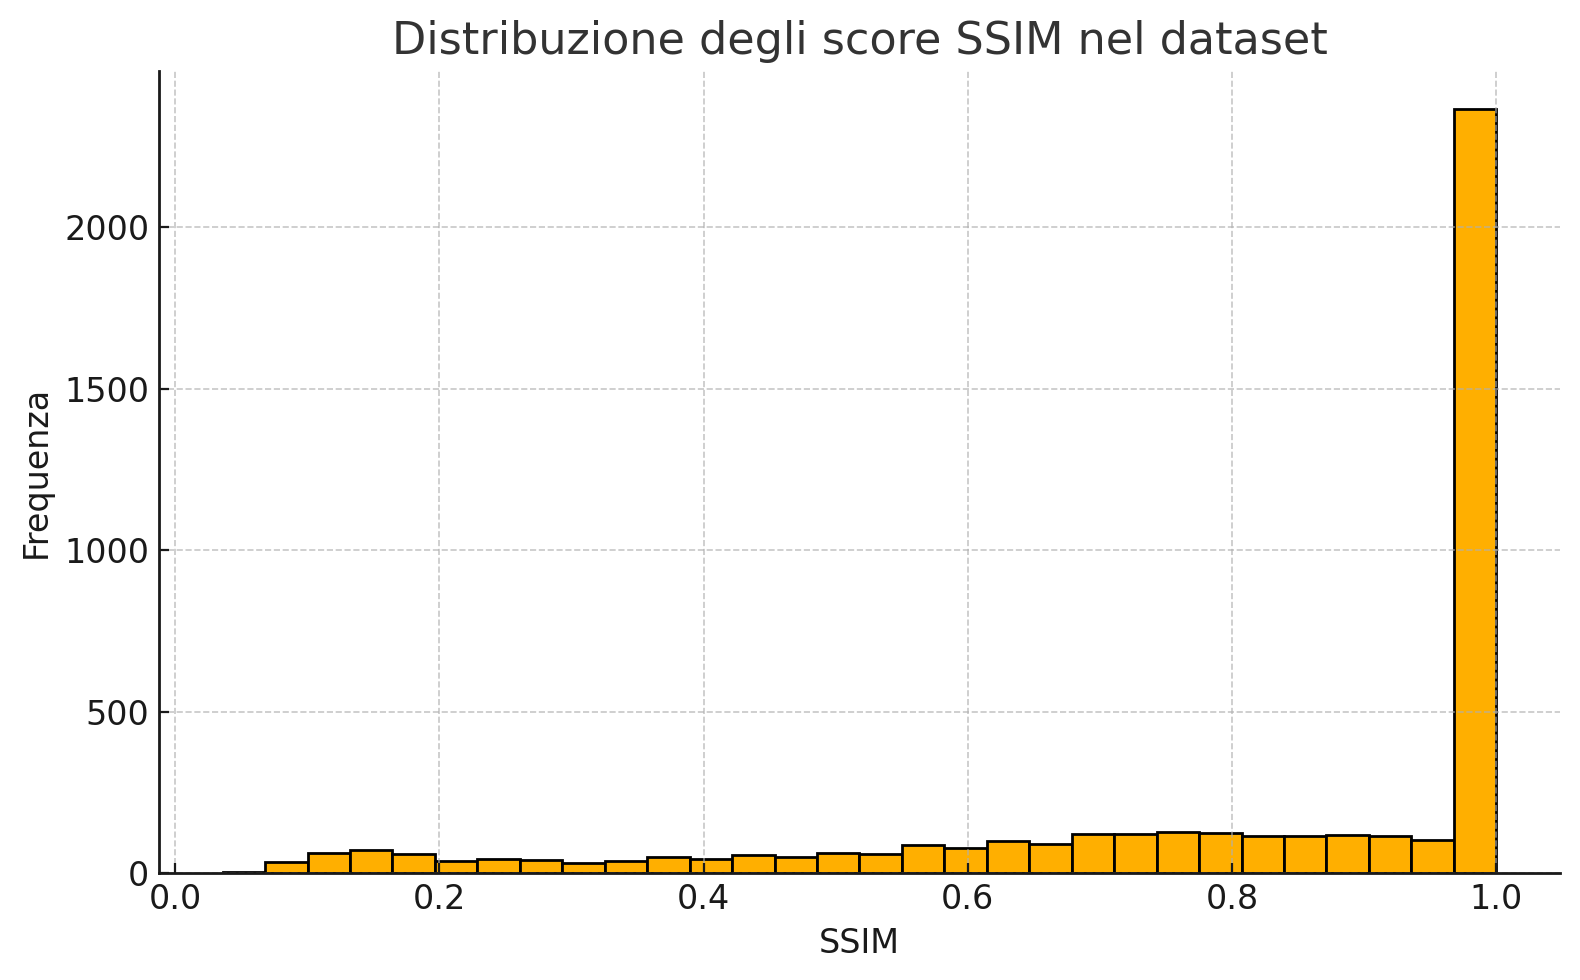
\includegraphics[width=0.8\textwidth]{imgs/ssim_distribution.png}
    \caption{Distribuzione dei valori SSIM nel dataset.}
    \label{fig:ssim_dist}
\end{figure}

Come illustrato nella Figura \ref{fig:ssim_dist}, il dataset mostra una copertura bilanciata di score SSIM distribuiti lungo tutto l’intervallo [0, 1]. La concentrazione di valori pari a 1.0 è intenzionale, in quanto corrisponde alle immagini originali confrontate con se stesse, utilizzate come riferimento assoluto per l’addestramento.
\section{Risultati dei Modelli}
\label{sec:risultati_regressione}

In questa sezione vengono confrontate le prestazioni dei tre modelli considerati: \textbf{ResNet50V2}, \textbf{MobileNetV2} e \textbf{EfficientNetB3}. Le metriche di regressione sono state calcolate su un sottoinsieme di test composto da 924 immagini.

\begin{table}[H]
    \centering
    \caption{Metriche di regressione per ciascun modello.}
    \label{tab:metriche_regressione}
    \begin{tabular}{lcccc}
        \toprule
        \textbf{Modello} & \textbf{R\textsuperscript{2}} & \textbf{MAE} & \textbf{MSE} & \textbf{RMSE} \\
        \midrule
        MobileNetV2     & 0.785 & 0.097 & 0.0218 & 0.1478 \\
        ResNet50V2      & 0.805 & 0.093 & 0.0196 & 0.1400 \\
        EfficientNetB3  & 0.813 & 0.091 & 0.0185 & 0.1360 \\
        \bottomrule
    \end{tabular}
\end{table}

\begin{figure}[H]
    \centering
    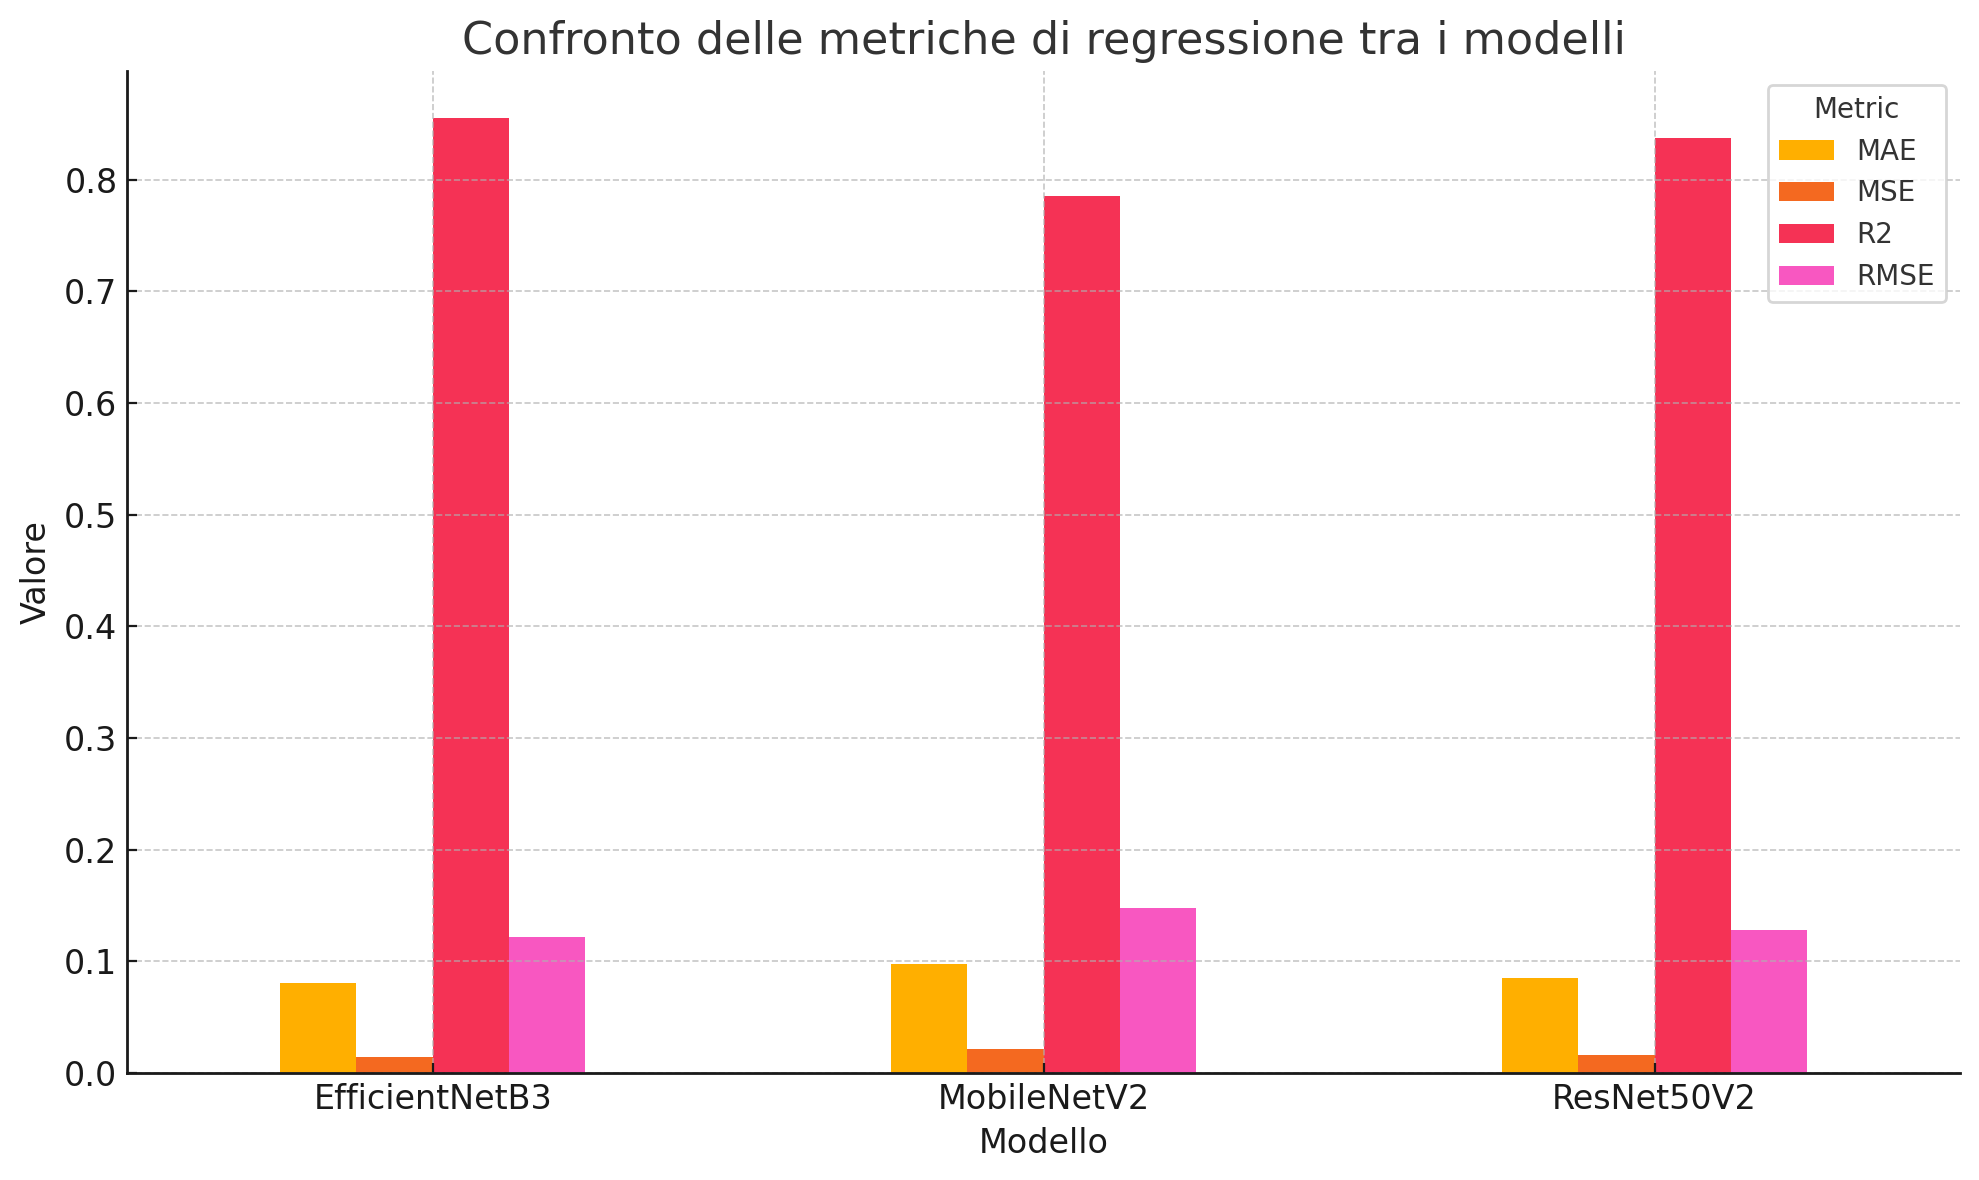
\includegraphics[width=0.9\textwidth]{imgs/regression_metrics_comparison.png}
    \caption{Confronto delle metriche di regressione tra i modelli.}
    \label{fig:metrics_comparison}
\end{figure}

Come mostrato nella Tabella \ref{tab:metriche_regressione} e nella Figura \ref{fig:metrics_comparison}, il modello \textbf{EfficientNetB3} si è rivelato il più performante tra i tre, con il valore più alto di $R^2$ (0.813) e il più basso errore medio assoluto (MAE) e quadratico medio (MSE). 

Segue il modello \textbf{ResNet50V2}, che offre comunque buoni risultati e una maggiore robustezza rispetto a MobileNetV2, ma con un errore leggermente superiore. \textbf{MobileNetV2}, pur avendo prestazioni inferiori, si dimostra comunque coerente e adeguato considerando la sua leggerezza computazionale, rendendolo un buon candidato per applicazioni su dispositivi a bassa potenza.

In generale, tutti e tre i modelli mostrano un'elevata capacità predittiva, con valori di $R^2$ superiori a 0.78, confermando l’efficacia dell’approccio proposto.
\section{Analisi Qualitativa delle Predizioni}
\label{sec:analisi_qualitativa}

Oltre alle metriche quantitative, è stato condotto un confronto qualitativo delle predizioni effettuate dai modelli su immagini soggette a diverse tipologie di degradazione. Ogni immagine è stata sottoposta a sei livelli crescenti di distorsione, partendo da una versione originale (sharp) fino ad arrivare a una versione fortemente degradata.

I modelli valutati sono \textbf{MobileNetV2}, \textbf{EfficientNetB3} e \textbf{ResNet50V2}. Per ciascuna trasformazione è stato registrato lo \textbf{score predetto} in corrispondenza di ogni livello di degrado.

\subsection{Motion Blur}
\begin{figure}[H]
    \centering
    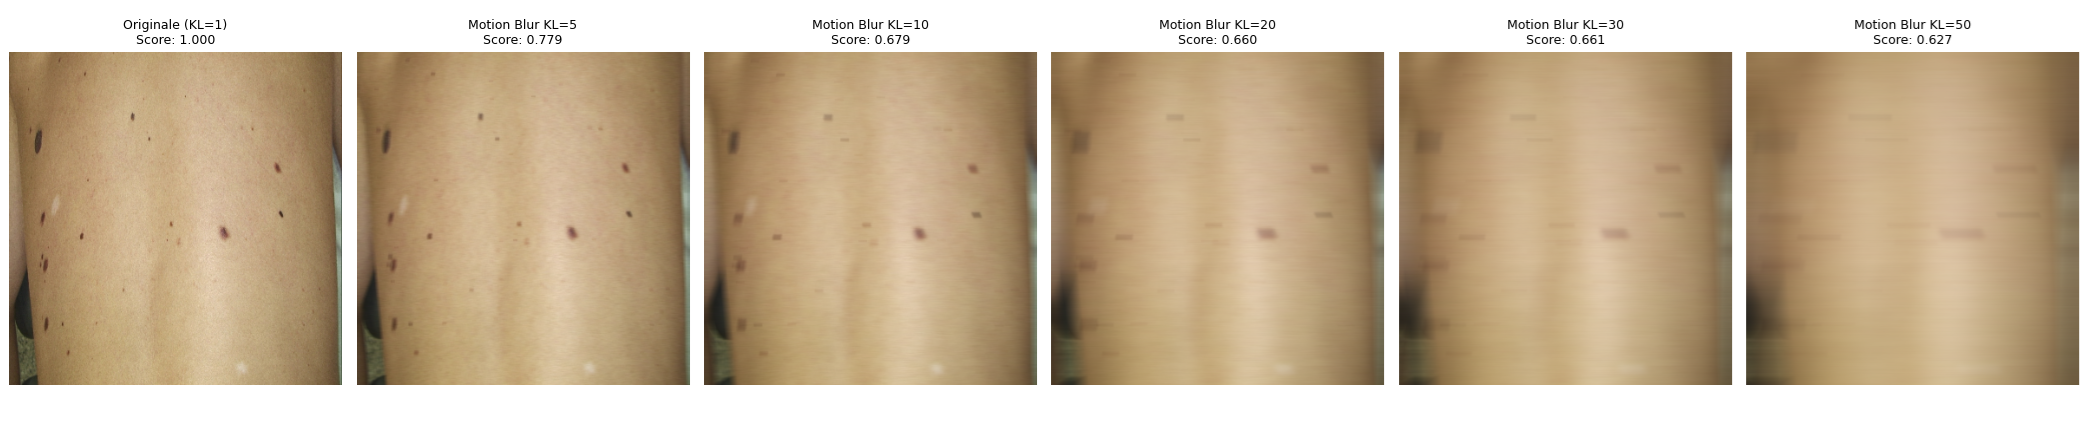
\includegraphics[width=\textwidth]{imgs/motionblur.png}
    \caption{Risultati su degradazione tramite motion blur.}
    \label{fig:motion_blur}
\end{figure}

\begin{table}[H]
\centering
\caption{Predizioni su immagini con degradazione Motion Blur}
\begin{tabular}{c|c|c|c|c}
\toprule
\textbf{Step} & \textbf{Kernel Size} & \textbf{MobileNetV2} & \textbf{EfficientNetB3} & \textbf{ResNet50V2} \\
\midrule
0 & 1  & 0.999 & 1.000 & 1.000 \\
1 & 5  & 0.796 & 0.779 & 0.952 \\
2 & 10 & 0.850 & 0.679 & 0.832 \\
3 & 20 & 0.892 & 0.660 & 0.820 \\
4 & 30 & 0.898 & 0.661 & 0.848 \\
5 & 50 & 0.897 & 0.627 & 0.864 \\
\bottomrule
\end{tabular}
\end{table}
Come visibile in Figura \ref{fig:motion_blur}, MobileNetV2 appare meno sensibile al peggioramento progressivo dell'immagine, con score elevati anche a livelli critici di blur. Al contrario, EfficientNetB3 evidenzia un calo più netto degli score, mostrando maggiore capacità di discriminazione visiva. ResNet50V2 mantiene un buon equilibrio tra sensibilità e stabilità.

\subsection{Pixelation}
\begin{figure}[H]
    \centering
    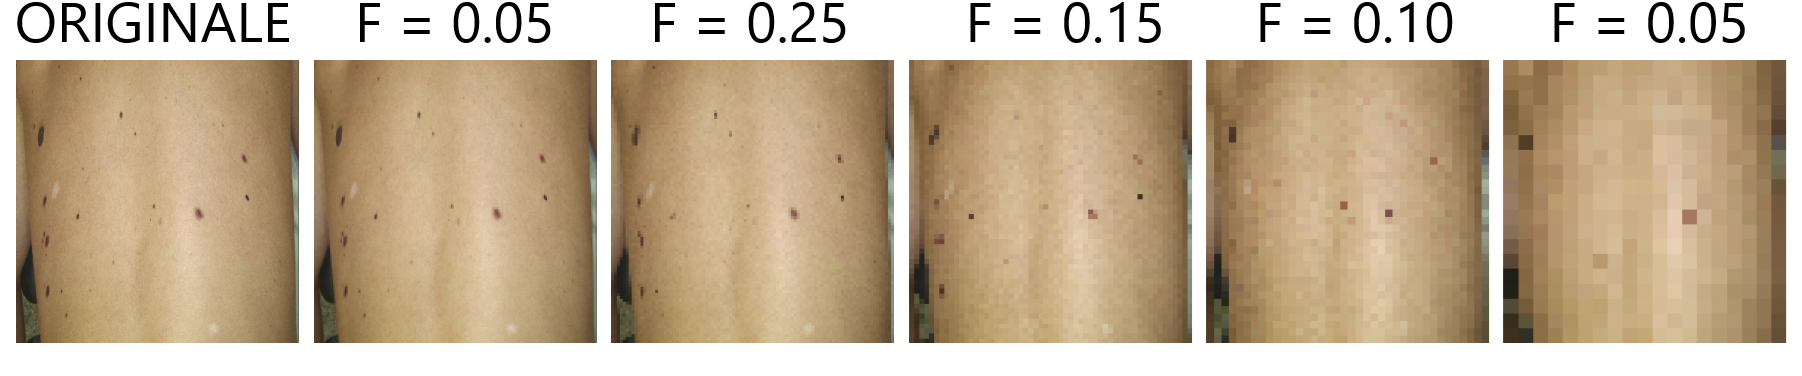
\includegraphics[width=\textwidth]{imgs/pixelation.png}
    \caption{Risultati su degradazione tramite pixelazione.}
    \label{fig:pixelation}
\end{figure}
\begin{table}[H]
\centering
\caption{Predizioni su immagini con degradazione tramite Pixelation}
\begin{tabular}{c|c|c|c|c}
\toprule
\textbf{Step} & \textbf{Fattore Pixelation} & \textbf{MobileNetV2} & \textbf{EfficientNetB3} & \textbf{ResNet50V2} \\
\midrule
0 & 1.00 & 1.000 & 0.999 & 1.000 \\
1 & 0.50 & 0.909 & 0.946 & 0.990 \\
2 & 0.25 & 0.733 & 0.831 & 0.902 \\
3 & 0.15 & 0.751 & 0.774 & 0.757 \\
4 & 0.10 & 0.687 & 0.842 & 0.714 \\
5 & 0.05 & 0.700 & 0.773 & 0.666 \\
\bottomrule
\end{tabular}
\end{table}
Nel caso della pixelazione (Figura \ref{fig:pixelation}), si nota una maggiore coerenza delle predizioni da parte di ResNet50V2, che riduce lo score in maniera progressiva e proporzionata. EfficientNetB3 mostra un comportamento simile. MobileNetV2, invece, presenta una curva meno regolare.

\subsection{Gaussian Blur}
\begin{figure}[H]
    \centering
    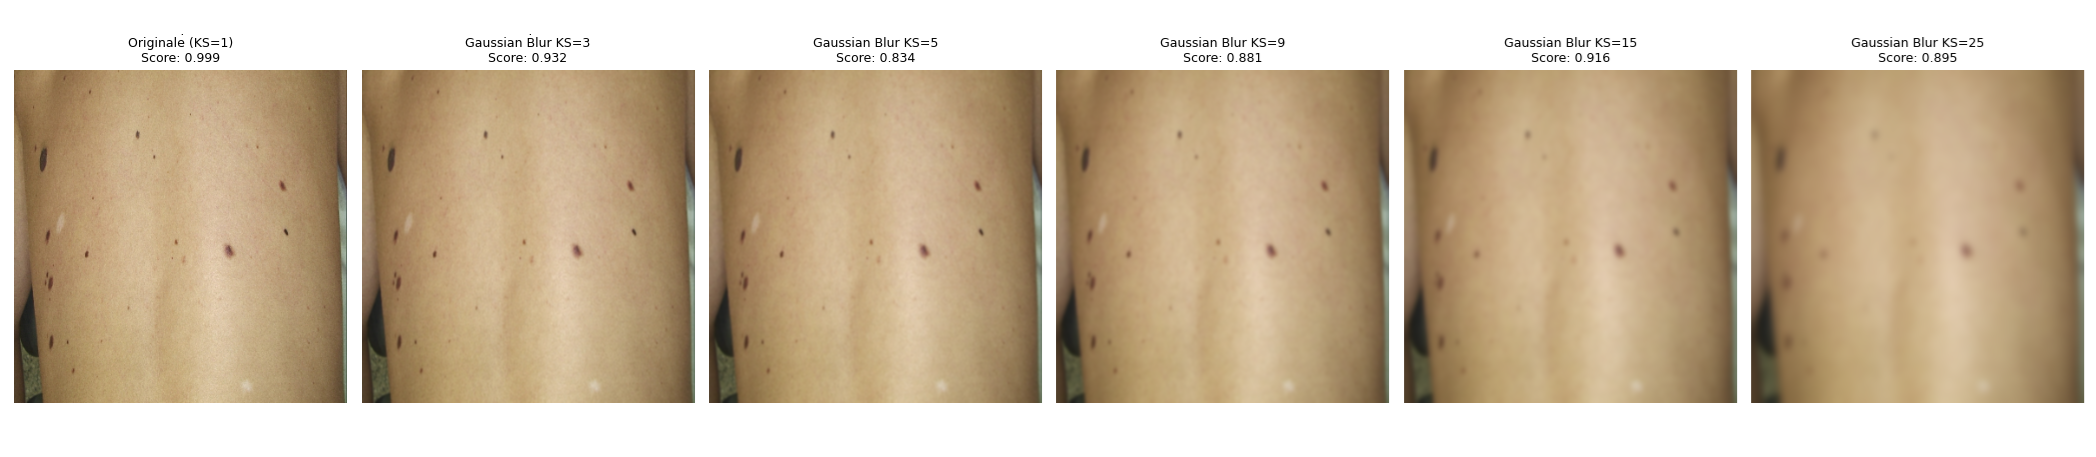
\includegraphics[width=\textwidth]{imgs/gaussianblur.png}
    \caption{Risultati su degradazione tramite gaussian blur.}
    \label{fig:gaussian_blur}
\end{figure}
\begin{table}[H]
\centering
\caption{Predizioni su immagini con Gaussian Blur}
\begin{tabular}{c|c|c|c|c}
\toprule
\textbf{Step} & \textbf{Kernel Size} & \textbf{MobileNetV2} & \textbf{EfficientNetB3} & \textbf{ResNet50V2} \\
\midrule
0 & 1  & 0.999 & 1.000 & 1.000 \\
1 & 3  & 0.932 & 0.978 & 0.993 \\
2 & 5  & 0.834 & 0.886 & 0.980 \\
3 & 9  & 0.881 & 0.771 & 0.922 \\
4 & 15 & 0.916 & 0.805 & 0.887 \\
5 & 25 & 0.895 & 0.706 & 0.865 \\
\bottomrule
\end{tabular}
\end{table}
Tutti i modelli rispondono in modo coerente al blur gaussiano (Figura \ref{fig:gaussian_blur}), con una decrescita fluida dello score. ResNet50V2 mantiene ancora una volta un'eccellente coerenza nella stima della qualità.

\subsection{Aberrazione Cromatica}
\begin{figure}[H]
    \centering
    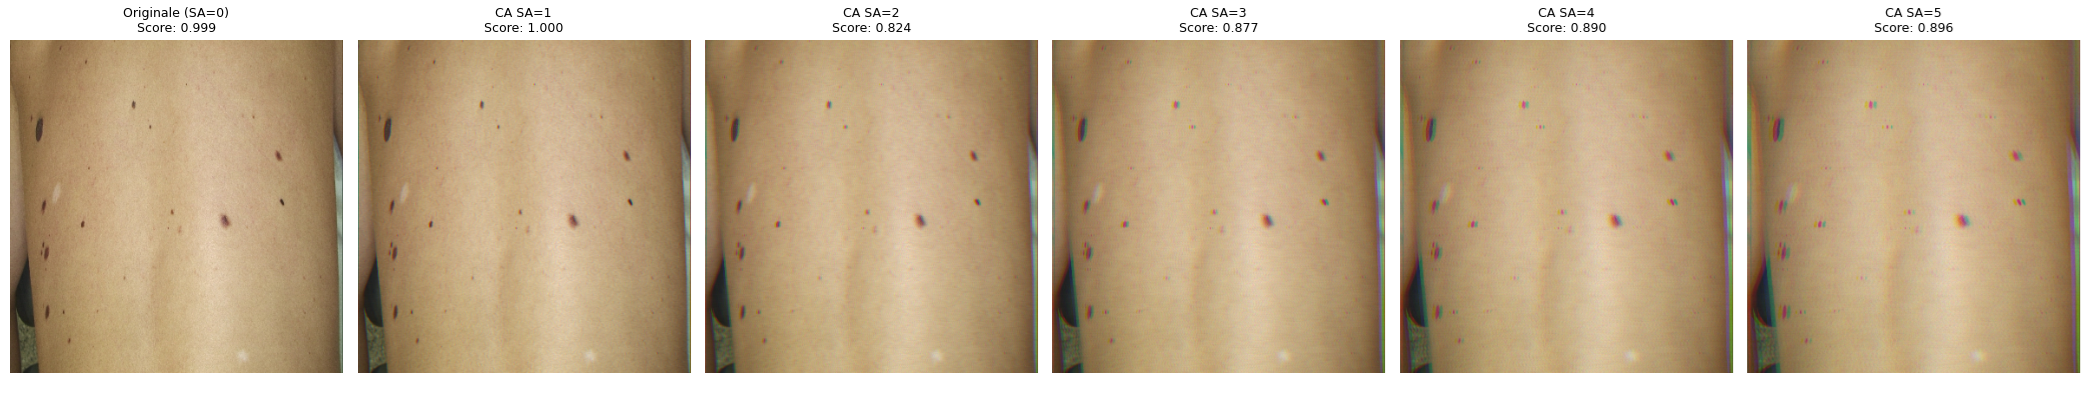
\includegraphics[width=\textwidth]{imgs/chromatic aberration.png}
    \caption{Risultati su aberrazione cromatica.}
    \label{fig:chromatic_aberration}
\end{figure}
\begin{table}[H]
\centering
\caption{Predizioni su immagini con aberrazione cromatica}
\begin{tabular}{c|c|c|c|c}
\toprule
\textbf{Step} & \textbf{Shift Aberrazione} & \textbf{MobileNetV2} & \textbf{EfficientNetB3} & \textbf{ResNet50V2} \\
\midrule
0 & 0   & 0.999 & 1.000 & 1.000 \\
1 & 1   & 1.000 & 0.978 & 0.991 \\
2 & 2.5 & 0.824 & 0.831 & 0.943 \\
3 & 3.5 & 0.877 & 0.733 & 0.916 \\
4 & 4   & 0.890 & 0.738 & 0.915 \\
5 & 5   & 0.896 & 0.779 & 0.911 \\
\bottomrule
\end{tabular}
\end{table}
Figura \ref{fig:chromatic_aberration} mostra che l’alterazione cromatica viene riconosciuta correttamente da tutti i modelli, ma in maniera differente. MobileNetV2 e ResNet50V2 tendono a mantenere score elevati anche in condizioni di forte aberrazione, mentre EfficientNetB3 risulta più conservativo nella valutazione.

\subsection{Rumore Additivo}
\begin{figure}[H]
    \centering
    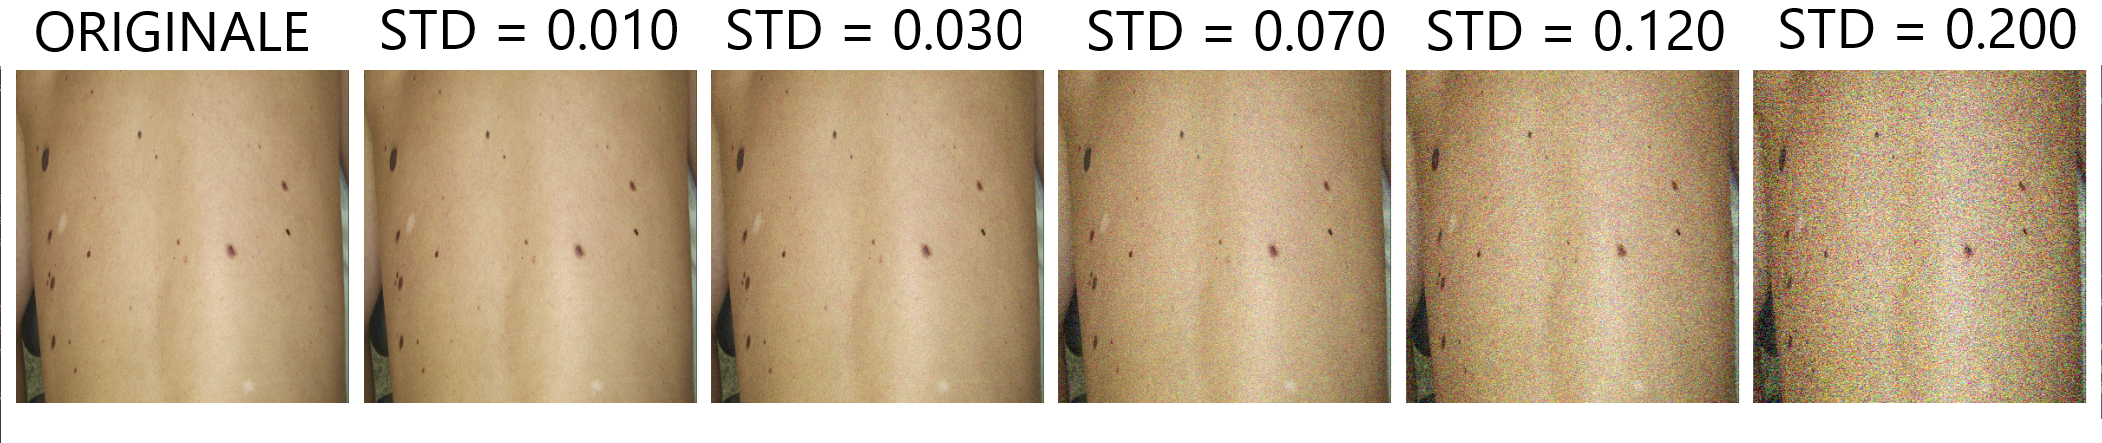
\includegraphics[width=\textwidth]{imgs/noisiness.png}
    \caption{Risultati su immagini degradate da rumore.}
    \label{fig:noise}
\end{figure}
\begin{table}[H]
\centering
\caption{Predizioni su immagini con rumore additivo}
\begin{tabular}{c|c|c|c|c}
\toprule
\textbf{Step} & \textbf{Deviazione Std} & \textbf{MobileNetV2} & \textbf{EfficientNetB3} & \textbf{ResNet50V2} \\
\midrule
0 & 0.000 & 0.999 & 1.000 & 1.000 \\
1 & 0.010 & 1.000 & 1.000 & 0.997 \\
2 & 0.030 & 0.993 & 0.831 & 0.985 \\
3 & 0.070 & 0.755 & 0.255 & 0.855 \\
4 & 0.120 & 0.310 & 0.105 & 0.267 \\
5 & 0.200 & 0.219 & 0.089 & 0.103 \\
\bottomrule
\end{tabular}
\end{table}
Infine, il test con rumore (Figura \ref{fig:noise}) evidenzia un comportamento eterogeneo. ResNet50V2 si distingue per la coerenza delle predizioni anche con elevata distorsione. EfficientNetB3 mostra un rapido crollo dello score, indicando una maggiore sensibilità. MobileNetV2 ha un comportamento intermedio, ma con alcune oscillazioni.

\bigskip
Nel complesso, i test qualitativi confermano quanto osservato nei risultati numerici: \textbf{EfficientNetB3} è il modello più sensibile ai cambiamenti, \textbf{ResNet50V2} offre le predizioni più stabili e coerenti, mentre \textbf{MobileNetV2}, pur essendo il più leggero, mantiene prestazioni accettabili in diversi scenari.
\section{Conclusioni}

L’analisi sia quantitativa che qualitativa ha dimostrato l’efficacia dell’approccio proposto per la stima automatica della qualità visiva delle immagini degradate. Tutti e tre i modelli testati sono riusciti ad apprendere una correlazione coerente tra le caratteristiche visive e il punteggio di qualità (SSIM), ma con comportamenti differenti.

\begin{itemize}
    \item \textbf{EfficientNetB3} si è rivelato il più sensibile e preciso, ma anche potenzialmente più esigente in termini computazionali.
    \item \textbf{ResNet50V2} ha offerto un buon compromesso tra accuratezza e stabilità, rendendolo adatto a scenari di uso reale.
    \item \textbf{MobileNetV2} ha mostrato prestazioni inferiori ma comunque interessanti, soprattutto per dispositivi a risorse limitate.
\end{itemize}

Questo modello può essere utilizzato come componente diagnostica in ambito dermatologico, come pre-filtro di qualità nei dataset medici, o integrato in pipeline di acquisizione per scartare immagini poco informative.


        %%%%%%%%%% CAPITOLO DI TESI %%%%%%%%%%
%
% Capitolo "5" 
%
%%%%%%%%%%%%%%%%%%%%%%%%%%%%%%%%%%%%%%
\chapter{Capitolo 5}
\label{chap:conclusioni}

Questo lavoro di tesi ha affrontato il problema della valutazione automatica della qualità delle immagini digitali in ambito dermatologico. L'obiettivo primario è stato sviluppare e validare un approccio basato su reti neurali convoluzionali (CNN) per fornire una stima \textit{no-reference} (cioè senza l'immagine originale) del livello di qualità di un'immagine.

A tal fine, è stato adottato un approccio basato sull'apprendimento profondo, sfruttando il Transfer Learning da architetture CNN pre-addestrate.

I risultati sperimentali, discussi nel Capitolo \ref{chap:esperimenti}, hanno dimostrato l'efficacia della metodologia. Tutti i modelli testati hanno appreso con successo a mappare le caratteristiche visive dell'immagine degradata a uno score di qualità, ottenendo buone prestazioni sul set di test (coefficiente R-squared R² > 0.78). In particolare, \textbf{EfficientNetB3} si è distinto per la maggiore precisione quantitativa (R²=0.813), mentre \textbf{ResNet50V2} ha mostrato un ottimo equilibrio tra accuratezza e stabilità delle predizioni di fronte a diversi tipi di degrado. Anche \textbf{MobileNetV2} ha fornito risultati interessanti, specialmente in ottica di efficienza computazionale.

Il contributo principale di questa tesi consiste quindi nell'aver sviluppato e validato uno strumento automatico ed efficace per la stima della qualità \textit{no-reference} di immagini dermatologiche. Tale strumento può avere significative ricadute pratiche:
\begin{itemize}
    \item Come \textbf{filtro di qualità} preliminare in sistemi di analisi automatica, per scartare input inaffidabili.
    \item Come \textbf{supporto in teledermatologia}, per fornire feedback sulla qualità dell'acquisizione.
    \item Per \textbf{standardizzare la qualità} all'interno di dataset medici per la ricerca.
\end{itemize}

Tra le \textbf{limitazioni} del lavoro vi sono la dipendenza dalla metrica SSIM come ground truth e la potenziale necessità di un dataset ancora più ampio e vario per coprire tutte le condizioni reali. Le \textbf{prospettive future} includono l'arricchimento del dataset (magari con valutazioni soggettive di esperti), l'esplorazione di architetture o task di apprendimento differenti, e la validazione del modello in contesti clinici reali, eventualmente ottimizzandolo per dispositivi a basse risorse.

In conclusione, questa tesi ha dimostrato con successo che le tecniche di deep learning possono superare i metodi tradizionali nella valutazione della qualità delle immagini dermatologiche, fornendo uno strumento promettente per migliorare l'affidabilità e l'efficienza dei processi diagnostici e di ricerca basati sull'imaging medico.

        %%%%%%%%%% CAPITOLO DI TESI %%%%%%%%%%
%
% Appendici 
%
%%%%%%%%%%%%%%%%%%%%%%%%%%%%%%%%%%%%%%
\mcchap{Appendici}{appendix:app1}

\section{Section}
Una sezione come le altre
    
        \appendix
        %%%%%%%%%% CAPITOLO DI TESI %%%%%%%%%%
%
% Colophon 
%
%%%%%%%%%%%%%%%%%%%%%%%%%%%%%%%%%%%%%%
\chapter*{Colophon}

La tesi è stata scritta utilizzando il linguaggio LaTeX.\\
Il template grafico è stato sviluppato da Carullo Moreno modifiche di Nicola Landro e Ignazio Gallo.\\
Il lavoro è stato svolto utilizzando il linguaggio di programmazione Java sul framework Android utilizzando l'ide Android Studio.\\
Le immagini sono state create appositamente con Gimp e Drawio, oppure sono degli screenshot di un dispositivo o emulatore.
    
    \backmatter{}

    %% Bibliografia
        \bibliography{biblio/biblio} 
        \bibliographystyle{ieeetr}

\end{document}
